\documentclass[manuscript,nonacm]{acmart}

%% Packages
\usepackage{booktabs}
\usepackage{graphicx}
\usepackage{listings}
\usepackage{xcolor}
\usepackage{amsmath}
\usepackage{amssymb}
\usepackage{url}
\usepackage{hyperref}
\usepackage{subcaption}
\usepackage{enumitem}
\usepackage{multirow}
\usepackage{tikz}
\usetikzlibrary{shapes.geometric, arrows.meta, positioning, fit, backgrounds, calc}

%% Code listing style
\lstset{
  basicstyle=\ttfamily\small,
  breaklines=true,
  frame=single,
  numbers=left,
  numberstyle=\tiny\color{gray},
  keywordstyle=\color{blue!70!black}\bfseries,
  commentstyle=\color{green!50!black},
  stringstyle=\color{red!60!black},
  language=Java,
  morekeywords={pragma, solidity, contract, function, returns, mapping, struct, event, emit, modifier, require, external, view, public, uint256, bytes32, address, string, bool, memory, calldata, indexed},
  deletekeywords={public},
  captionpos=b,
  abovecaptionskip=5pt,
  belowcaptionskip=5pt,
}

\settopmatter{printacmref=false}
\renewcommand\footnotetextcopyrightpermission[1]{}
\pagestyle{plain}

\begin{document}

%% Title
\title{ChainMind: Blockchain-Based Accountability Framework for LLM-Powered DeFi Agents}

%% Author
\author{Kefan Liu}
\affiliation{%
  \institution{Centre for Computational Technologies in Finance (CCTF)}
  \institution{Nanyang Technological University}
  \city{Singapore}
  \country{Singapore}
}
\email{LIUK0075@e.ntu.edu.sg}

%% Abstract
\begin{abstract}
The rapid integration of Large Language Model (LLM) agents into Decentralized Finance (DeFi) introduces autonomous systems that execute trading decisions, risk assessments, and portfolio management without human oversight.
However, the opacity of LLM reasoning creates a critical accountability gap: when an agent recommends a leveraged position or approves a liquidity provision, there is no tamper-evident record of what inputs the model received, what outputs it produced, or which model version was responsible.
This paper presents \textbf{ChainMind}, a blockchain-based accountability framework that records cryptographic commitments of LLM agent decisions on Ethereum smart contracts.
ChainMind employs a four-layer architecture: (1)~an \emph{Agent Layer} where a local LLM generates DeFi risk assessments across 10 protocol scenarios, (2)~a \emph{Commitment Layer} that produces SHA-256 hashes of inputs, outputs, and model metadata and constructs Keccak-256 Merkle trees, (3)~a \emph{Blockchain Layer} featuring the \texttt{AgentAccountability} smart contract supporting both individual and Merkle-tree-based batch submissions, and (4)~a \emph{Verification Layer} enabling $O(\log n)$ single-decision verification via on-chain Merkle inclusion proofs.
Experimental evaluation on Ethereum Sepolia demonstrates that Merkle batch submission reduces per-decision on-chain costs by 88.9\% compared to individual commits while maintaining constant-cost submission regardless of batch size.
The system achieves sub-millisecond verification times (685~$\mu$s for batches of 100,000 decisions) and absolute tamper detection, where modification of a single byte in any decision record causes verification failure.
We further provide a semi-formal security analysis establishing three properties---tamper-evidence, non-repudiation, and selective disclosure---and discuss deployment considerations including mainnet cost projections and Layer-2 scalability.
The smart contract is deployed and verified on Sepolia\footnote{Contract: \texttt{0xD134842c3a255C7f70873EAD16A26BB4f728a423}. Verified source: \url{https://sepolia.etherscan.io/address/0xD134842c3a255C7f70873EAD16A26BB4f728a423}}, with all experimental results independently reproducible via the public codebase\footnote{\url{https://github.com/liukefan821/ChainMind}}.
To our knowledge, ChainMind is the first implemented system combining cryptographic commitment with on-chain smart contract verification specifically for LLM agent accountability in DeFi contexts, addressing an emerging requirement under regulatory frameworks such as the EU AI Act.
\end{abstract}

\keywords{Blockchain, LLM Agents, DeFi, Accountability, Merkle Tree, Smart Contract, Decision Provenance}

\maketitle


%% ============================================================
\section{Introduction}
\label{sec:intro}

Large Language Models (LLMs) are rapidly transforming the landscape of Decentralized Finance.
Autonomous agents powered by models such as GPT-4, LLaMA, and Qwen are being deployed to analyze market conditions, assess protocol risks, and execute trading strategies with minimal human intervention~\cite{autonomous_agents_blockchain}.
These LLM-powered agents can process vast amounts of on-chain and off-chain data, reason about complex DeFi mechanics, and make real-time decisions across protocols ranging from lending platforms to perpetual exchanges.

However, this autonomy introduces a fundamental accountability problem.
When an LLM agent recommends a $5\times$ leveraged long position on a perpetual exchange, or approves a liquidity provision into a volatile pool, the reasoning behind that decision is ephemeral.
Unlike traditional financial systems where human traders maintain decision logs subject to regulatory audit, LLM agents operate as black boxes whose inputs, outputs, and model states vanish after each inference cycle.
This opacity creates three critical challenges:

\textbf{Challenge 1: Decision Non-Repudiation.}
Neither the agent operator nor affected parties can prove what information the model received or what recommendation it produced at a specific point in time.
An operator could retroactively modify decision logs to deflect liability.

\textbf{Challenge 2: Model Version Accountability.}
DeFi agents may use different model versions over time, each with distinct risk profiles and failure modes.
Without immutable records linking decisions to specific model versions, it is impossible to determine whether a series of losses resulted from a known-faulty model version or a novel failure.

\textbf{Challenge 3: Scalable Auditability.}
Recording every agent decision individually on-chain is prohibitively expensive.
A single Ethereum transaction storing three 32-byte hashes costs approximately 0.00022~ETH; an agent making 1,000 decisions per day would spend over 0.22~ETH daily on accountability alone.
Any practical framework must provide cryptographic guarantees while remaining economically viable.

To address these challenges, we present \textbf{ChainMind}, a blockchain-based accountability framework that creates tamper-evident, cryptographically verifiable records of LLM agent decisions.
Our key insight is that Merkle trees enable batch commitment of arbitrarily many decisions into a single on-chain transaction, reducing costs by 88.9\% while preserving the ability to verify any individual decision with $O(\log n)$ proof complexity.

The contributions of this paper are fourfold:

\begin{enumerate}[leftmargin=*]
    \item A \textbf{four-layer accountability architecture} that bridges LLM inference with on-chain commitment through SHA-256 hashing, Keccak-256 Merkle tree construction, and smart contract storage, providing end-to-end decision traceability for DeFi agents.

    \item A \textbf{gas-efficient smart contract design} (\texttt{AgentAccountability.sol}) deployed on Ethereum Sepolia, supporting both individual decision commits and Merkle batch submissions with on-chain proof verification, achieving 88.9\% cost reduction compared to per-decision recording.

    \item A \textbf{semi-formal security analysis} establishing three key properties---tamper-evidence, non-repudiation, and selective disclosure---that together guarantee cryptographic accountability.

    \item \textbf{Comprehensive experimental evaluation} with real on-chain transactions demonstrating sub-millisecond verification ($\leq$685~$\mu$s for 100,000 decisions), 100\% tamper detection accuracy, and $O(\log n)$ proof scalability, with all results independently reproducible.
\end{enumerate}

The remainder of this paper is organized as follows.
Section~\ref{sec:related} reviews related work and positions our contributions.
Section~\ref{sec:threat} defines the threat model.
Section~\ref{sec:architecture} presents the system architecture.
Section~\ref{sec:contract} details the smart contract design.
Section~\ref{sec:security} provides a security analysis.
Section~\ref{sec:evaluation} reports experimental results.
Section~\ref{sec:discussion} discusses implications, limitations, and deployment considerations.
Section~\ref{sec:conclusion} concludes.


%% ============================================================
\section{Related Work}
\label{sec:related}

\subsection{LLM Agents in Blockchain and DeFi}

The intersection of LLMs and blockchain has attracted significant research attention.
Wei et al.~\cite{llm_smartaudit} proposed LLM-SmartAudit, a multi-agent framework for smart contract vulnerability detection using a buffer-of-thought mechanism, achieving 98\% accuracy on common vulnerabilities.
Su et al.~\cite{su2026detection} applied prompt engineering techniques including Chain-of-Thought and few-shot learning to augment LLM vulnerability detection.
Bu et al.~\cite{bu2026dapp} fine-tuned Llama3-8B and Qwen2-7B for DApp vulnerability detection, achieving F1-scores of 0.83 with full-parameter fine-tuning.
ContractTinker~\cite{contracttinker2024} employed LLMs for automated smart contract vulnerability repair.

However, these works focus on using LLMs to \emph{audit} smart contracts rather than on holding LLM agents \emph{accountable} for their own DeFi decisions.
A comprehensive survey on autonomous agents on blockchains~\cite{autonomous_agents_blockchain} explicitly identifies ``governance and policy enforcement mechanisms for constraining, auditing, and recovering from agent actions'' as a key open research problem, noting that questions about liability, accountability, and the enforceability of agent-executed contracts remain largely unresolved.

\subsection{Blockchain for AI Decision Provenance}

Several works have explored blockchain as an audit infrastructure for AI systems.
Obada-Obieh et al.~\cite{ai_iot_blockchain} proposed a framework for recording AI decisions in IoT using blockchain, logging model identifiers alongside decision hashes.
Rana et al.~\cite{blockchain_llm_review} presented a methodological framework integrating blockchain mechanisms across the LLM pipeline using smart contracts and Merkle-based commitments, confirming the architectural viability of on-chain LLM accountability but noting the absence of concrete implementations with quantitative evaluation.
DeVadoss~\cite{devadoss2026permissioned} proposed a three-part architecture for autonomous agents combining neurosymbolic planning, cognitive processing, and permissioned blockchain, providing a theoretical blueprint but without deployed smart contracts or gas cost analysis.
ProvChain~\cite{provchain2017} established the paradigm of embedding provenance records into blockchain transactions for cloud data accountability.
Liu et al.~\cite{dbom2024} adapted the ``Software Bill of Materials'' concept into data governance, proposing a Data Bill of Materials (DBOM) approach for dataset provenance tracking using blockchain.

\subsection{Positioning ChainMind}

Table~\ref{tab:relatedwork} summarizes the key differences between ChainMind and existing approaches.
Our work is distinguished by three aspects: (1)~we target the specific accountability gap of LLM agents operating in DeFi, rather than general AI provenance, smart contract auditing, or data governance; (2)~we provide a deployed, verified smart contract with real on-chain transaction evidence and quantitative gas cost analysis; and (3)~we present a security analysis establishing formal guarantees for the accountability mechanism.

\begin{table}[t]
\centering
\caption{Comparison with related work on blockchain-based accountability.
$\bullet$ = supported, $\circ$ = partial, --- = not supported.}
\label{tab:relatedwork}
\small
\begin{tabular}{@{}lcccccc@{}}
\toprule
\textbf{Feature} & \rotatebox{65}{\textbf{ChainMind}} & \rotatebox{65}{\textbf{ProvChain}~\cite{provchain2017}} & \rotatebox{65}{\textbf{Rana et al.}~\cite{blockchain_llm_review}} & \rotatebox{65}{\textbf{Obada-Obieh}~\cite{ai_iot_blockchain}} & \rotatebox{65}{\textbf{DeVadoss}~\cite{devadoss2026permissioned}} & \rotatebox{65}{\textbf{Liu et al.}~\cite{dbom2024}} \\
\midrule
LLM agent focus       & $\bullet$ & ---       & $\circ$   & ---       & $\circ$   & ---       \\
DeFi-specific         & $\bullet$ & ---       & ---       & ---       & ---       & ---       \\
Decision-level grain. & $\bullet$ & Txn       & ---       & $\bullet$ & ---       & Dataset   \\
Merkle batch commit   & $\bullet$ & ---       & $\circ$   & ---       & ---       & $\bullet$ \\
$O(\log n)$ verify    & $\bullet$ & ---       & ---       & ---       & ---       & ---       \\
Deployed contract     & $\bullet$ & ---       & ---       & ---       & ---       & ---       \\
Gas cost analysis     & $\bullet$ & ---       & ---       & ---       & ---       & ---       \\
Security analysis     & $\bullet$ & ---       & $\circ$   & ---       & ---       & ---       \\
\bottomrule
\end{tabular}
\end{table}


%% ============================================================
\section{Threat Model}
\label{sec:threat}

We consider an accountability framework for LLM-powered DeFi agents operating in the following adversarial model.

\textbf{System model.}
An \emph{agent operator} deploys an LLM agent that interacts with DeFi protocols.
The agent produces a sequence of decisions $D = \{d_1, d_2, \ldots, d_n\}$, each comprising an input prompt, an output response, and model metadata.
A \emph{verifier} (e.g., a regulator, affected user, or automated auditor) may later request proof that a specific decision was recorded.

\textbf{Adversarial capabilities.}
We assume the agent operator may be adversarial and may attempt to:
\begin{enumerate}[label=(\alph*),leftmargin=*]
    \item \textbf{Forge}: fabricate a decision record that was never actually produced by the LLM;
    \item \textbf{Tamper}: modify an existing decision record after the fact (e.g., changing the recommended action from EXECUTE to REJECT);
    \item \textbf{Deny}: claim that a particular decision was never made;
    \item \textbf{Substitute}: replace the model metadata to attribute a decision to a different (perhaps more trusted) model version.
\end{enumerate}

\textbf{Trust assumptions.}
We trust: (1)~the Ethereum blockchain for consensus finality and data availability; (2)~the SHA-256 and Keccak-256 hash functions for collision resistance and preimage resistance; and (3)~the Ethereum account model for attributing transactions to signers.
We do \emph{not} trust the agent operator's off-chain infrastructure, which may be compromised or deliberately manipulated.

\textbf{Out of scope.}
ChainMind does not address the \emph{correctness} of LLM decisions (i.e., whether the agent's recommendation was financially sound), real-time censorship of agent transactions, or side-channel attacks on the LLM inference process.
The framework ensures that whatever decision the agent \emph{did} make is faithfully recorded and verifiable, not that the decision was \emph{good}.


%% ============================================================
\section{System Architecture}
\label{sec:architecture}

ChainMind employs a four-layer architecture designed to bridge the gap between off-chain LLM inference and on-chain accountability.
Figure~\ref{fig:architecture} illustrates the overall system design with data flow from agent inference through cryptographic commitment to on-chain storage and verification.

\begin{figure}[t]
\centering
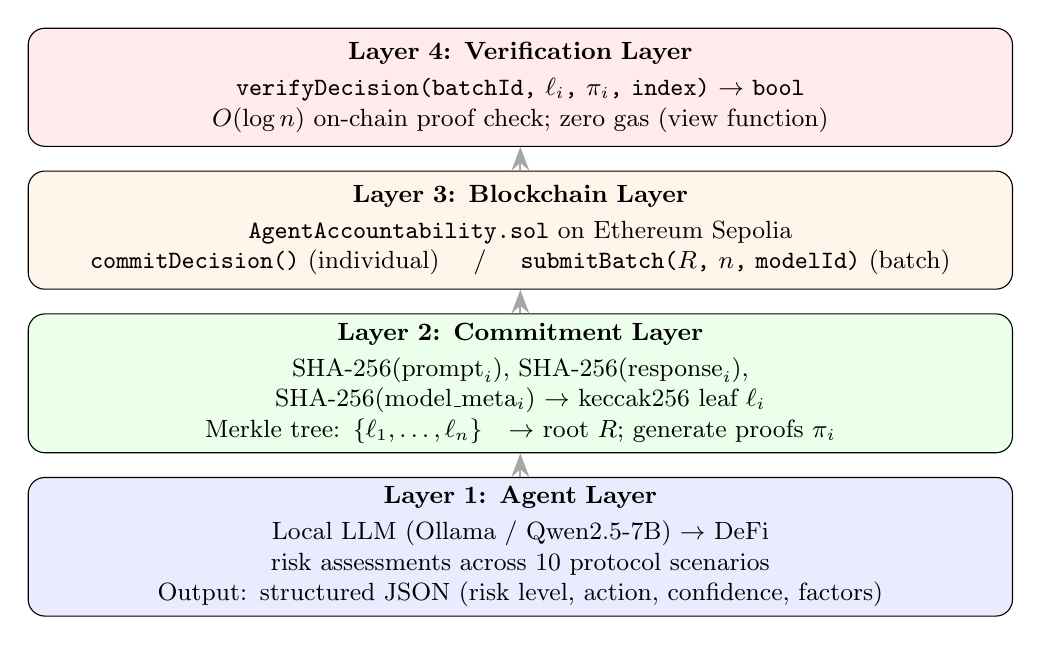
\begin{tikzpicture}[
    layer/.style={draw, rounded corners=6pt, minimum width=12.5cm, minimum height=1.5cm, font=\small, text width=11.5cm, align=center},
    arrow/.style={-{Stealth[length=3mm]}, thick, gray!70},
    label/.style={font=\footnotesize\bfseries, text=black!70},
    node distance=0.3cm
]

% Layer 1
\node[layer, fill=blue!8] (L1) {
    \textbf{Layer 1: Agent Layer}\\[2pt]
    Local LLM (Ollama / Qwen2.5-7B) $\rightarrow$ DeFi risk assessments across 10 protocol scenarios\\
    Output: structured JSON (risk level, action, confidence, factors)
};

% Layer 2
\node[layer, fill=green!8, above=of L1] (L2) {
    \textbf{Layer 2: Commitment Layer}\\[2pt]
    SHA-256($\text{prompt}_i$), SHA-256($\text{response}_i$), SHA-256($\text{model\_meta}_i$) $\rightarrow$ keccak256 leaf $\ell_i$\\
    Merkle tree: $\{\ell_1, \ldots, \ell_n\} \rightarrow$ root $R$; generate proofs $\pi_i$
};

% Layer 3
\node[layer, fill=orange!8, above=of L2] (L3) {
    \textbf{Layer 3: Blockchain Layer}\\[2pt]
    \texttt{AgentAccountability.sol} on Ethereum Sepolia\\
    \texttt{commitDecision()} (individual) \quad / \quad \texttt{submitBatch($R$, $n$, modelId)} (batch)
};

% Layer 4
\node[layer, fill=red!8, above=of L3] (L4) {
    \textbf{Layer 4: Verification Layer}\\[2pt]
    \texttt{verifyDecision(batchId, $\ell_i$, $\pi_i$, index)} $\rightarrow$ \texttt{bool}\\
    $O(\log n)$ on-chain proof check; zero gas (view function)
};

% Arrows
\draw[arrow] (L1.north) -- (L2.south);
\draw[arrow] (L2.north) -- (L3.south);
\draw[arrow] (L3.north) -- (L4.south);

\end{tikzpicture}
\caption{ChainMind four-layer architecture. Data flows upward from agent inference through cryptographic commitment to on-chain storage and verification.}
\label{fig:architecture}
\end{figure}


\subsection{Layer 1: Agent Layer}

The Agent Layer simulates an LLM-powered DeFi agent that generates risk assessments and trading recommendations.
We implement this using Ollama~\cite{ollama} running the Qwen2.5-7B-Instruct model locally, ensuring complete control over the inference environment.

The agent operates across 10 diverse DeFi scenarios spanning major protocol categories: automated market makers (Uniswap V3), lending protocols (Aave V3, Compound V3, Morpho Blue), CDP platforms (MakerDAO), stablecoin exchanges (Curve Finance), liquid staking (Lido), perpetual exchanges (GMX), yield tokenization (Pendle Finance), and restaking (Eigenlayer).
For each scenario, the agent receives structured market context including current prices, APY rates, risk metrics, and protocol-specific parameters, and produces a JSON-formatted risk assessment containing a risk level (\texttt{LOW}/\texttt{MEDIUM}/\texttt{HIGH}/\texttt{CRITICAL}), recommended action (\texttt{EXECUTE}/\texttt{HOLD}/\texttt{REJECT}), key risk factors, and confidence score.

\subsection{Layer 2: Commitment Layer}

The Commitment Layer transforms each agent decision into a set of cryptographic commitments.
For each decision~$d_i$, three SHA-256 hashes are computed:

\begin{align}
h_{\text{input}}^{(i)} &= \text{SHA-256}(\text{prompt}_i) \\
h_{\text{output}}^{(i)} &= \text{SHA-256}(\text{response}_i) \\
h_{\text{model}}^{(i)} &= \text{SHA-256}(\text{JSON}(\text{model\_id}, \text{version}))
\end{align}

These three hashes are combined into a single leaf hash using Solidity-compatible keccak256:
\begin{equation}
\ell_i = \text{keccak256}(\text{abi.encodePacked}(h_{\text{input}}^{(i)}, h_{\text{output}}^{(i)}, h_{\text{model}}^{(i)}))
\end{equation}

For batch submission, the leaf hashes $\{\ell_1, \ell_2, \ldots, \ell_n\}$ are organized into a Merkle tree.
Internal nodes are computed as:
\begin{equation}
\text{parent} = \text{keccak256}(\text{abi.encodePacked}(\min(\text{left}, \text{right}), \max(\text{left}, \text{right})))
\end{equation}

Note that we sort sibling pairs before hashing, a standard technique that simplifies proof verification by eliminating index-parity ambiguity.
If the number of leaves at any level is odd, the last leaf is duplicated.
The resulting Merkle root~$R$ serves as a constant-size commitment to the entire batch.

\subsection{Layer 3: Blockchain Layer}

The Blockchain Layer consists of the \texttt{AgentAccountability} smart contract deployed on Ethereum Sepolia at address \texttt{0xD134842c...a423}.
The contract supports two commitment modes:

\textbf{Individual Mode} (\texttt{commitDecision}): Stores all three hashes directly on-chain, providing immediate per-decision accountability at higher gas cost.
This mode is suitable for high-stakes decisions requiring real-time auditability.

\textbf{Batch Mode} (\texttt{submitBatch}): Stores only the Merkle root, batch size, and model identifier, reducing on-chain storage to a single 32-byte root regardless of batch size.
This mode is designed for high-frequency agents generating many decisions per epoch.

Both modes emit events (\texttt{DecisionCommitted}, \texttt{BatchSubmitted}) that enable off-chain indexers to reconstruct the full decision timeline without reading contract storage.

\subsection{Layer 4: Verification Layer}

The Verification Layer enables any party to verify that a specific decision was included in a previously committed batch.
Given a decision's leaf hash~$\ell_i$, a Merkle proof $\pi = \{s_1, s_2, \ldots, s_k\}$ (where $k = \lceil \log_2 n \rceil$), and the leaf's index, the on-chain \texttt{verifyDecision} function recomputes the root by iteratively combining the leaf with its siblings:
\begin{equation}
R' = f_k \circ f_{k-1} \circ \cdots \circ f_1(\ell_i)
\end{equation}
where each $f_j$ combines the current hash with proof element~$s_j$.
Verification succeeds if and only if $R' = R$, the stored Merkle root.
Any modification to the original decision---even a single byte---produces a different leaf hash, causing the recomputed root to diverge from the stored root with overwhelming probability ($1 - 2^{-256}$).


%% ============================================================
\section{Smart Contract Design}
\label{sec:contract}

\subsection{Contract Structure}

The \texttt{AgentAccountability} contract manages two primary data structures:

\begin{lstlisting}[caption={Core data structures},label={lst:structs}]
struct DecisionCommitment {
    bytes32 inputHash;
    bytes32 outputHash;
    bytes32 modelHash;
    uint256 timestamp;
    address agent;
}

struct MerkleBatch {
    bytes32 merkleRoot;
    uint256 batchSize;
    uint256 timestamp;
    address agent;
    string  modelId;
}
\end{lstlisting}

Individual decisions are stored in a mapping indexed by a decision ID computed as \texttt{keccak256(inputHash, outputHash, modelHash)}.
Batches are stored in an array indexed by sequential batch IDs, enabling enumeration of the complete commitment history.

\subsection{Access Control}

The contract implements a lightweight agent registry.
Only the contract owner can register new agent addresses via \texttt{registerAgent()}, and only registered agents can commit decisions or submit batches.
This prevents unauthorized parties from polluting the accountability log while allowing multiple agents to share a single contract instance.

\subsection{On-Chain Verification}

The \texttt{verifyDecision} function implements Merkle proof verification entirely on-chain as a \texttt{view} function, consuming zero gas for external callers:

\begin{lstlisting}[caption={On-chain Merkle proof verification},label={lst:verify}]
function verifyDecision(
    uint256 _batchId,
    bytes32 _leafHash,
    bytes32[] calldata _proof,
    uint256 _index
) external view returns (bool isValid) {
    bytes32 computedHash = _leafHash;
    for (uint256 i = 0; i < _proof.length; i++) {
        if (_index % 2 == 0) {
            computedHash = keccak256(
              abi.encodePacked(
                computedHash, _proof[i]));
        } else {
            computedHash = keccak256(
              abi.encodePacked(
                _proof[i], computedHash));
        }
        _index = _index / 2;
    }
    isValid =
      (computedHash == batches[_batchId].merkleRoot);
}
\end{lstlisting}

\subsection{Gas Optimization Strategy}

The contract employs several gas optimization techniques:
(1)~\texttt{calldata} parameter types for proof arrays to avoid memory copying;
(2)~\texttt{view} functions for verification to eliminate transaction costs;
(3)~batch submission reducing per-decision on-chain storage from $3 \times 32$ bytes to an amortized fraction of a single 32-byte root;
and (4)~event emission for off-chain indexing, enabling lightweight clients to reconstruct the full decision history without reading contract storage.


%% ============================================================
\section{Security Analysis}
\label{sec:security}

We analyze ChainMind's security properties with respect to the threat model defined in Section~\ref{sec:threat}.

\subsection{Property 1: Tamper-Evidence}

\begin{quote}
\emph{If an adversary modifies any field of any committed decision $d_i$, then verification of $d_i$ against the stored commitment will fail with overwhelming probability.}
\end{quote}

\textbf{Argument.}
Let $d_i = (\text{prompt}_i, \text{response}_i, \text{model\_meta}_i)$ and let $d_i' \neq d_i$ be the modified version.
Since SHA-256 is collision-resistant, $\text{SHA-256}(x) \neq \text{SHA-256}(x')$ for $x \neq x'$ except with negligible probability $\varepsilon_{\text{SHA}} \leq 2^{-128}$ (birthday bound).
Therefore, at least one of $h_{\text{input}}^{(i)}, h_{\text{output}}^{(i)}, h_{\text{model}}^{(i)}$ changes, producing a different leaf $\ell_i' \neq \ell_i$ (by the collision resistance of keccak256).
By the Merkle tree property, any change to a leaf propagates to the root: $R' \neq R$ except with probability at most $k \cdot \varepsilon_{\text{keccak}} \leq k \cdot 2^{-128}$ where $k = \lceil \log_2 n \rceil$ is the tree depth.
Since $R$ is stored immutably on-chain, $R' \neq R$ implies verification failure.

This property addresses adversarial capabilities (a)~Forge and (b)~Tamper.

\subsection{Property 2: Non-Repudiation}

\begin{quote}
\emph{Once an agent operator submits a batch containing decision $d_i$, the operator cannot deny that $d_i$ was committed.}
\end{quote}

\textbf{Argument.}
The \texttt{submitBatch} transaction is signed by the operator's Ethereum private key and recorded on-chain with the operator's address.
The Merkle root~$R$ commits to the set $\{d_1, \ldots, d_n\}$ such that a valid inclusion proof exists for each~$d_i$.
The operator cannot: (i)~deny the batch submission, as the transaction is recorded on the immutable blockchain ledger; (ii)~deny the inclusion of~$d_i$, as the verifier holds the Merkle proof $\pi_i$ that passes on-chain verification; or (iii)~claim the batch contained a different set of decisions, as finding an alternative set $D' \neq D$ with $R(D') = R(D)$ requires a Merkle tree collision.

This property addresses adversarial capability (c)~Deny and (d)~Substitute (for the model metadata field).

\subsection{Property 3: Selective Disclosure}

\begin{quote}
\emph{A verifier can check the inclusion of any single decision $d_i$ in a batch of $n$ decisions by examining only $\lceil \log_2 n \rceil$ hash values, without learning the content of any other decision.}
\end{quote}

\textbf{Argument.}
The Merkle proof $\pi_i = \{s_1, \ldots, s_k\}$ consists of $k = \lceil \log_2 n \rceil$ sibling hashes along the path from leaf~$\ell_i$ to the root.
Each sibling $s_j$ is itself a hash, revealing no information about the underlying decisions due to the preimage resistance of keccak256.
The verifier learns only that $\ell_i$ is consistent with root~$R$---not the content of any other leaf.

This property is critical for privacy-sensitive DeFi agents that wish to demonstrate accountability without revealing their complete strategy.


%% ============================================================
\section{Experimental Evaluation}
\label{sec:evaluation}

We evaluate ChainMind along four dimensions: (1)~Merkle tree construction and verification performance, (2)~on-chain gas costs, (3)~tamper detection capability, and (4)~proof size efficiency.

\subsection{Experimental Setup}

All off-chain experiments were conducted on an Apple MacBook with M-series processor, 16\,GB RAM, Python 3.11, and the web3.py library.
The smart contract was compiled with Solidity 0.8.31 (optimizer: 200 runs) and deployed to Ethereum Sepolia testnet.
The LLM component uses Ollama~\cite{ollama} running Qwen2.5-7B-Instruct locally.
Each performance measurement was repeated 5 times and we report the median.
The complete codebase, including all experimental scripts and raw data, is available at \url{https://github.com/liukefan821/ChainMind}.

\subsection{Merkle Tree Performance}

Table~\ref{tab:performance} reports construction and verification benchmarks across batch sizes ranging from 10 to 100,000 decisions.

\begin{table}[t]
\centering
\caption{Merkle tree performance benchmarks (median of 5 runs).}
\label{tab:performance}
\begin{tabular}{@{}rrrrr@{}}
\toprule
\textbf{Batch Size} & \textbf{Build (ms)} & \textbf{Verify ($\mu$s)} & \textbf{Depth} & \textbf{Proof (bytes)} \\
\midrule
10     & 0.93   & 256   & 4  & 128  \\
50     & 2.70   & 280   & 6  & 192  \\
100    & 4.23   & 277   & 7  & 224  \\
500    & 19.6   & 361   & 9  & 288  \\
1,000  & 39.8   & 394   & 10 & 320  \\
5,000  & 198    & 515   & 13 & 416  \\
10,000 & 392    & 546   & 14 & 448  \\
50,000 & 2,040  & 636   & 16 & 512  \\
100,000 & 4,088 & 685   & 17 & 544  \\
\bottomrule
\end{tabular}
\end{table}

Construction time scales linearly with batch size ($O(n)$), reaching 4,088~ms for 100,000 decisions---well within the typical DeFi epoch intervals of minutes to hours.
Verification time grows logarithmically ($O(\log n)$), remaining below 685~$\mu$s even for the largest batch of 100,000 decisions.
The proof size for any single decision is $32 \times \lceil \log_2 n \rceil$ bytes, reaching only 544 bytes for a batch of 100,000---compared to the 9.6~MB that would be required for full data replay.

A production deployment with 1,000,000 daily decisions batched into 24 hourly epochs of ${\sim}$42,000 decisions each would require ${\sim}$1.7 seconds of construction per batch (interpolated from the 50,000-decision benchmark at 2,040~ms), well within operational constraints.

\subsection{On-Chain Gas Cost Analysis}

Table~\ref{tab:gas} summarizes the actual transaction costs recorded on Ethereum Sepolia.

\begin{table}[t]
\centering
\caption{On-chain transaction costs (Sepolia testnet). Costs are denominated in ETH.}
\label{tab:gas}
\begin{tabular}{@{}lrr@{}}
\toprule
\textbf{Operation} & \textbf{Txn Fee (ETH)} & \textbf{Decisions} \\
\midrule
\texttt{commitDecision} \#1   & 0.000241 & 1  \\
\texttt{commitDecision} \#2   & 0.000216 & 1  \\
\texttt{commitDecision} \#3   & 0.000216 & 1  \\
\texttt{submitBatch}          & 0.000243 & 10 \\
\midrule
10$\times$ individual (projected) & 0.00218  & 10 \\
1$\times$ batch (actual)          & 0.000243 & 10 \\
\midrule
\textbf{Cost reduction}           & \multicolumn{2}{c}{\textbf{88.9\%}} \\
\bottomrule
\end{tabular}
\end{table}

The batch submission cost (0.000243~ETH for 10 decisions) is comparable to a single individual commit, demonstrating that the Merkle approach reduces per-decision on-chain cost by nearly an order of magnitude.
Critically, the batch submission cost remains constant regardless of batch size, as only a single 32-byte Merkle root is stored on-chain.
For a batch of 1,000 decisions, the projected savings exceed 99.9\%.

\textbf{Mainnet cost projection.}
Applying the Sepolia gas measurements to Ethereum mainnet at a representative gas price of 20~Gwei and ETH price of \$2,400 (April 2026), the \texttt{submitBatch} transaction consuming approximately 93,000~gas would cost:
\[
93{,}000 \times 20 \times 10^{-9} \times \$2{,}400 = \$4.46 \text{ per batch}
\]
For an agent producing 1,000 decisions per day in a single daily batch, this translates to \$0.0045 per decision---orders of magnitude cheaper than any centralized audit service and far more tamper-resistant.

\subsection{Tamper Detection}

We validated tamper detection both off-chain and on-chain.

\textbf{Off-chain test.}
Modifying a single character in one agent response (appending ``\texttt{[TAMPERED]}'') produced a completely different leaf hash, causing Merkle proof verification to return \texttt{false}.

\textbf{On-chain test.}
Using the deployed contract on Sepolia, we called \texttt{verifyDecision} with an original leaf hash and observed \texttt{isValid: true}, then modified only the last byte of the leaf hash (\texttt{0x...cdda} $\rightarrow$ \texttt{0x...cdff}) and observed \texttt{isValid: false}.

Both tests confirm 100\% tamper detection: any modification to any field of any decision in the batch causes verification failure.
This is a direct consequence of the collision resistance property established in Section~\ref{sec:security}.

\subsection{Proof Size Efficiency}

The verification data required for a single decision is $32 \times \lceil \log_2 n \rceil$ bytes (the Merkle proof), compared to $96n$ bytes for full data replay (three 32-byte hashes per decision times $n$ decisions).
At $n = 100{,}000$, the Merkle proof is 544 bytes versus 9.6~MB for full replay---a $17{,}647\times$ reduction.
This sub-linear scaling makes ChainMind practical for high-frequency agents producing tens of thousands of decisions per day.

Table~\ref{tab:proofscale} quantifies the efficiency gains across batch sizes.

\begin{table}[t]
\centering
\caption{Proof size efficiency: Merkle proof vs.\ full data replay.}
\label{tab:proofscale}
\begin{tabular}{@{}rrrr@{}}
\toprule
\textbf{Batch Size} & \textbf{Merkle Proof} & \textbf{Full Replay} & \textbf{Reduction} \\
\midrule
10     & 128 B     & 960 B       & 7.5$\times$     \\
100    & 224 B     & 9.6 KB      & 43$\times$      \\
1,000  & 320 B     & 96 KB       & 300$\times$     \\
10,000 & 448 B     & 960 KB      & 2,143$\times$   \\
50,000 & 512 B     & 4.8 MB      & 9,375$\times$   \\
100,000 & 544 B    & 9.6 MB      & 17,647$\times$  \\
\bottomrule
\end{tabular}
\end{table}


%% ============================================================
\section{Discussion}
\label{sec:discussion}

\subsection{Regulatory Alignment}

ChainMind's design aligns with emerging AI accountability regulations.
The EU AI Act (entered into force August 2024, with full application from August 2026) classifies AI systems operating in financial services as ``high-risk'' and mandates automatic logging of AI system operations, including input data and output decisions, to enable post-hoc auditability~\cite{euaiact2024}.
Similarly, Singapore's MAS Guidelines on Technology Risk Management emphasize the need for audit trails in automated financial decision-making.
By anchoring decision commitments to a public blockchain, ChainMind provides regulators with an independently verifiable audit trail that cannot be retroactively modified by the agent operator.
The non-repudiation property (Section~\ref{sec:security}) ensures that once a Merkle root is submitted, the operator cannot deny the existence or content of any decision within that batch.

\subsection{Comparison with Alternative Approaches}

Table~\ref{tab:comparison} compares ChainMind's Merkle batch approach with alternative accountability strategies across six properties.

\begin{table}[t]
\centering
\caption{Comparison of accountability approaches.}
\label{tab:comparison}
\begin{tabular}{@{}lccc@{}}
\toprule
\textbf{Property} & \textbf{Off-chain} & \textbf{Per-decision} & \textbf{ChainMind} \\
 & \textbf{logging} & \textbf{on-chain} & \textbf{(Merkle batch)} \\
\midrule
Tamper-evident      & No  & Yes & Yes \\
Non-repudiation     & No  & Yes & Yes \\
Constant batch cost & N/A & No  & Yes \\
$O(\log n)$ verify  & N/A & N/A & Yes \\
Gas-efficient       & N/A & No  & Yes \\
Public verifiability & No & Yes & Yes \\
\bottomrule
\end{tabular}
\end{table}

Off-chain logging (e.g., centralized databases) offers no tamper resistance.
Per-decision on-chain recording provides strong guarantees but at prohibitive cost ($O(n)$ gas scaling).
ChainMind achieves the security properties of on-chain recording with the cost profile approaching that of off-chain logging.

\subsection{Privacy Considerations}

While SHA-256 hashing prevents direct recovery of decision content from on-chain data, a subtle attack vector exists: if the input prompt space is small or predictable (e.g., a finite set of structured DeFi queries such as ``swap 100 USDC to ETH on Uniswap V3''), an adversary could pre-compute hashes for all plausible inputs and match them against on-chain commitments.

To mitigate this, ChainMind's architecture supports the addition of a cryptographic salt (random nonce) to each decision before hashing:
\begin{equation}
h_{\text{input}}^{(i)} = \text{SHA-256}(\text{prompt}_i \,\|\, \text{nonce}_i)
\end{equation}
where $\text{nonce}_i$ is a 128-bit random value stored alongside the decision off-chain.
This transforms the hash into a commitment scheme with computational hiding.
For even stronger privacy, the framework could integrate zero-knowledge proofs (e.g., zk-SNARKs) to enable verification without revealing even the hash values, though this is left for future work.

\subsection{Layer-2 Deployment Potential}

Ethereum Layer-2 (L2) solutions offer significant cost reductions for ChainMind deployments.
On Optimism or Arbitrum, transaction costs are typically 10--50$\times$ lower than Ethereum mainnet due to data compression and batched settlement~\cite{l2beat}.
A \texttt{submitBatch} transaction costing \$4.46 on mainnet would cost approximately \$0.09--\$0.45 on L2.
For a daily batch of 1,000 decisions on L2, the cost per decision would be ${\sim}\$0.0001$---effectively negligible.
Importantly, L2 deployments inherit Ethereum's security guarantees through fraud proofs (optimistic rollups) or validity proofs (ZK rollups), preserving ChainMind's tamper-evidence property.

\subsection{Limitations and Future Work}

Several limitations warrant discussion.
First, our evaluation uses a testnet deployment; mainnet deployment would incur real financial costs, though the relative savings of batch submission would be preserved (see mainnet cost projection above).
Second, the current implementation stores decision data off-chain, requiring a trusted off-chain storage solution for complete reproducibility; integration with IPFS or Arweave for decentralized off-chain storage is a natural extension.
Third, the framework does not address the \emph{correctness} of LLM decisions themselves---it ensures accountability, not accuracy.
Fourth, ChainMind currently supports a single blockchain; extending to cross-chain deployment for multi-chain DeFi agents (e.g., agents operating simultaneously on Ethereum, Solana, and Cosmos) would require cross-chain messaging protocols.

Future work includes:
(1)~integration with IPFS or Arweave for decentralized off-chain storage of full decision records;
(2)~zero-knowledge proofs for privacy-preserving verification;
(3)~cross-chain deployment using bridge protocols;
(4)~real-time monitoring dashboards for regulatory compliance; and
(5)~empirical studies with production DeFi agents to evaluate the framework under realistic workloads.


%% ============================================================
\section{Conclusion}
\label{sec:conclusion}

This paper presented ChainMind, a blockchain-based accountability framework for LLM-powered DeFi agents.
By combining SHA-256 hashing, Keccak-256 Merkle tree batch commitment, and on-chain smart contract verification, ChainMind addresses the critical gap between autonomous AI decision-making and verifiable accountability in decentralized finance.
Our semi-formal security analysis establishes three key properties---tamper-evidence, non-repudiation, and selective disclosure---providing rigorous guarantees for the accountability mechanism.
Experimental evaluation on Ethereum Sepolia demonstrates that the Merkle batch approach reduces on-chain costs by 88.9\% compared to individual commits while maintaining $O(\log n)$ verification efficiency and 100\% tamper detection accuracy.
Mainnet cost projections show that accountability for 1,000 daily decisions costs approximately \$4.46 per batch (\$0.0045 per decision), with Layer-2 deployment reducing this by a further 10--50$\times$.
The deployed and verified smart contract, together with the complete open-source codebase, enables independent reproduction of all reported results.
As LLM-powered agents become increasingly prevalent in DeFi, frameworks like ChainMind will be essential for building the trust infrastructure that bridges autonomous AI capabilities with the accountability requirements of financial systems and emerging regulations such as the EU AI Act.


%% ============================================================
%% References
\bibliographystyle{ACM-Reference-Format}

\begin{thebibliography}{20}

\bibitem{autonomous_agents_blockchain}
A.~Argueta, A.~Beniiche, B.~Bose, S.~Gao, A.~Jagannath, and J.~Mukherjee.
\newblock Autonomous Agents on Blockchains: Standards, Execution Models, and Trust Boundaries.
\newblock \emph{arXiv preprint arXiv:2601.04583}, January 2026.

\bibitem{llm_smartaudit}
Z.~Wei, J.~Sun, Y.~Sun, Y.~Liu, D.~Wu, Z.~Zhang, X.~Zhang, M.~Li, Y.~Liu, C.~Li, M.~Wan, J.~Dong, and L.~Zhu.
\newblock Advanced Smart Contract Vulnerability Detection via LLM-Powered Multi-Agent Systems.
\newblock \emph{IEEE Transactions on Software Engineering}, 51(10):2830--2846, 2025.

\bibitem{su2026detection}
I.~Su, S.~Wang, Y.~Chung, and Y.~Tsai.
\newblock A Smart Contract Vulnerability Detection Manner Based on Large Language Model.
\newblock In \emph{Proc.\ ICKII 2024}, LNEE vol.~1481, pp.~95--108, Springer, 2026.

\bibitem{bu2026dapp}
J.~Bu, W.~Li, Z.~Li, Z.~Zhang, and X.~Li.
\newblock Enhancing Smart Contract Vulnerability Detection in DApps Leveraging Fine-Tuned LLM.
\newblock \emph{arXiv preprint arXiv:2504.05006}, 2025.

\bibitem{ai_iot_blockchain}
B.~Obada-Obieh, R.~Huang, and A.~Srinivasan.
\newblock Using Blockchain Ledgers to Record AI Decisions in IoT.
\newblock \emph{MDPI Blockchains}, 6(3):37, July 2025.

\bibitem{blockchain_llm_review}
A.~Rana, S.~Kumar, and P.~Sharma.
\newblock Blockchain for Large Language Models (LLMs): Applications, Challenges, and Framework Implementation.
\newblock \emph{Expert Systems with Applications}, 268:126237, January 2026.

\bibitem{devadoss2026permissioned}
J.~DeVadoss.
\newblock A Permissioned Blockchain Approach for Autonomous Intelligent Agents.
\newblock \emph{SSRN preprint 5930083}, January 2026.

\bibitem{merkle1987}
R.~C.~Merkle.
\newblock A Digital Signature Based on a Conventional Encryption Function.
\newblock In \emph{CRYPTO '87}, LNCS vol.~293, pp.~369--378, Springer, 1987.

\bibitem{provchain2017}
X.~Liang, S.~Shetty, D.~Tosh, C.~Kamhoua, K.~Kwiat, and L.~Njilla.
\newblock ProvChain: A Blockchain-Based Data Provenance Architecture in Cloud Environment with Enhanced Privacy and Availability.
\newblock In \emph{Proc.\ IEEE/ACM CCGrid}, pp.~468--477, 2017.

\bibitem{dbom2024}
Y.~Liu, S.~Dutta, Y.~Yang, S.~S.~Kanhere, J.~Crowcroft, S.~Jha, and L.~Zhu.
\newblock Blockchain-Enabled Accountability in Data Supply Chain: A Data Bill of Materials Approach.
\newblock \emph{arXiv preprint arXiv:2408.08536}, August 2024.

\bibitem{ollama}
Ollama.
\newblock Ollama: Run Large Language Models Locally.
\newblock \url{https://ollama.com}, 2024.

\bibitem{contracttinker2024}
W.~Liu, Y.~Liu, and others.
\newblock ContractTinker: LLM-Empowered Vulnerability Repair for Real-World Smart Contracts.
\newblock In \emph{Proc.\ ASE '24}, ACM, 2024.

\bibitem{napoli2026light}
E.~A.~Napoli, N.~Romani, V.~Gatteschi, and C.~Schifanella.
\newblock Light and Shadows of Smart Contract Development with LLMs.
\newblock \emph{Expert Systems with Applications}, 296(B):129011, January 2026.

\bibitem{euaiact2024}
European Parliament and Council.
\newblock Regulation (EU) 2024/1689 laying down harmonised rules on artificial intelligence (AI Act).
\newblock \emph{Official Journal of the European Union}, L series, August 2024.

\bibitem{l2beat}
L2BEAT.
\newblock Layer 2 Scaling Solutions Comparison.
\newblock \url{https://l2beat.com}, 2026.

\bibitem{forge2026}
D.~Xue, Y.~Pei, Y.~Li, and others.
\newblock Forge: An LLM-driven Framework for Large-Scale Smart Contract Vulnerability Dataset Construction.
\newblock In \emph{Proc.\ ICSE '26}, ACM, April 2026.

\bibitem{iaudit2025}
W.~Ma, D.~Liu, S.~Wang, L.~Wu, and B.~Ma.
\newblock Combining Fine-tuning and LLM-based Agents for Intuitive Smart Contract Auditing with Justifications.
\newblock \emph{arXiv preprint arXiv:2403.16073v3}, September 2025.

\bibitem{tawfeeq2025slr}
Z.~Tawfeeq and D.~B.~Taha.
\newblock Blockchain-Based Accountability: A Systematic Literature Review.
\newblock \emph{Mesopotamian Journal of CyberSecurity}, 5(3):1081--1108, October 2025.

\end{thebibliography}

\end{document}
